\documentclass[twoside]{book}

% Packages required by doxygen
\usepackage{fixltx2e}
\usepackage{calc}
\usepackage{doxygen}
\usepackage{graphicx}
\usepackage[utf8]{inputenc}
\usepackage{makeidx}
\usepackage{multicol}
\usepackage{multirow}
\PassOptionsToPackage{warn}{textcomp}
\usepackage{textcomp}
\usepackage[nointegrals]{wasysym}
\usepackage[table]{xcolor}

% Font selection
\usepackage[T1]{fontenc}
\usepackage{mathptmx}
\usepackage[scaled=.90]{helvet}
\usepackage{courier}
\usepackage{amssymb}
\usepackage{sectsty}
\renewcommand{\familydefault}{\sfdefault}
\allsectionsfont{%
  \fontseries{bc}\selectfont%
  \color{darkgray}%
}
\renewcommand{\DoxyLabelFont}{%
  \fontseries{bc}\selectfont%
  \color{darkgray}%
}
\newcommand{\+}{\discretionary{\mbox{\scriptsize$\hookleftarrow$}}{}{}}

% Page & text layout
\usepackage{geometry}
\geometry{%
  a4paper,%
  top=2.5cm,%
  bottom=2.5cm,%
  left=2.5cm,%
  right=2.5cm%
}
\tolerance=750
\hfuzz=15pt
\hbadness=750
\setlength{\emergencystretch}{15pt}
\setlength{\parindent}{0cm}
\setlength{\parskip}{0.2cm}
\makeatletter
\renewcommand{\paragraph}{%
  \@startsection{paragraph}{4}{0ex}{-1.0ex}{1.0ex}{%
    \normalfont\normalsize\bfseries\SS@parafont%
  }%
}
\renewcommand{\subparagraph}{%
  \@startsection{subparagraph}{5}{0ex}{-1.0ex}{1.0ex}{%
    \normalfont\normalsize\bfseries\SS@subparafont%
  }%
}
\makeatother

% Headers & footers
\usepackage{fancyhdr}
\pagestyle{fancyplain}
\fancyhead[LE]{\fancyplain{}{\bfseries\thepage}}
\fancyhead[CE]{\fancyplain{}{}}
\fancyhead[RE]{\fancyplain{}{\bfseries\leftmark}}
\fancyhead[LO]{\fancyplain{}{\bfseries\rightmark}}
\fancyhead[CO]{\fancyplain{}{}}
\fancyhead[RO]{\fancyplain{}{\bfseries\thepage}}
\fancyfoot[LE]{\fancyplain{}{}}
\fancyfoot[CE]{\fancyplain{}{}}
\fancyfoot[RE]{\fancyplain{}{\bfseries\scriptsize Generated on Fri Sep 12 2014 00\+:40\+:16 for S\+S\+C Arduino Interface by Doxygen }}
\fancyfoot[LO]{\fancyplain{}{\bfseries\scriptsize Generated on Fri Sep 12 2014 00\+:40\+:16 for S\+S\+C Arduino Interface by Doxygen }}
\fancyfoot[CO]{\fancyplain{}{}}
\fancyfoot[RO]{\fancyplain{}{}}
\renewcommand{\footrulewidth}{0.4pt}
\renewcommand{\chaptermark}[1]{%
  \markboth{#1}{}%
}
\renewcommand{\sectionmark}[1]{%
  \markright{\thesection\ #1}%
}

% Indices & bibliography
\usepackage{natbib}
\usepackage[titles]{tocloft}
\setcounter{tocdepth}{3}
\setcounter{secnumdepth}{5}
\makeindex

% Hyperlinks (required, but should be loaded last)
\usepackage{ifpdf}
\ifpdf
  \usepackage[pdftex,pagebackref=true]{hyperref}
\else
  \usepackage[ps2pdf,pagebackref=true]{hyperref}
\fi
\hypersetup{%
  colorlinks=true,%
  linkcolor=blue,%
  citecolor=blue,%
  unicode%
}

% Custom commands
\newcommand{\clearemptydoublepage}{%
  \newpage{\pagestyle{empty}\cleardoublepage}%
}


%===== C O N T E N T S =====

\begin{document}

% Titlepage & ToC
\hypersetup{pageanchor=false,
             bookmarks=true,
             bookmarksnumbered=true,
             pdfencoding=unicode
            }
\pagenumbering{roman}
\begin{titlepage}
\vspace*{7cm}
\begin{center}%
{\Large S\+S\+C Arduino Interface \\[1ex]\large 1.\+0 }\\
\vspace*{1cm}
{\large Generated by Doxygen 1.8.8}\\
\vspace*{0.5cm}
{\small Fri Sep 12 2014 00:40:16}\\
\end{center}
\end{titlepage}
\clearemptydoublepage
\tableofcontents
\clearemptydoublepage
\pagenumbering{arabic}
\hypersetup{pageanchor=true}

%--- Begin generated contents ---
\chapter{Interface}
\label{md__r_e_a_d_m_e}
\hypertarget{md__r_e_a_d_m_e}{}
Arduino Code for the S\+S\+C Drill project. 
\chapter{Hierarchical Index}
\section{Class Hierarchy}
This inheritance list is sorted roughly, but not completely, alphabetically\+:\begin{DoxyCompactList}
\item \contentsline{section}{Csv\+Writer}{\pageref{class_csv_writer}}{}
\item Q\+Dialog\begin{DoxyCompactList}
\item \contentsline{section}{progress\+Dialog}{\pageref{classprogress_dialog}}{}
\item \contentsline{section}{Variable\+Editor}{\pageref{class_variable_editor}}{}
\end{DoxyCompactList}
\item Q\+Main\+Window\begin{DoxyCompactList}
\item \contentsline{section}{Main\+Window}{\pageref{class_main_window}}{}
\end{DoxyCompactList}
\end{DoxyCompactList}

\chapter{Class Index}
\section{Class List}
Here are the classes, structs, unions and interfaces with brief descriptions\+:\begin{DoxyCompactList}
\item\contentsline{section}{\hyperlink{class_csv_writer}{Csv\+Writer} \\*For simple csv output }{\pageref{class_csv_writer}}{}
\item\contentsline{section}{\hyperlink{class_main_window}{Main\+Window} \\*The \hyperlink{class_main_window}{Main\+Window} class. Actually is the heart of the interface. All the methods which deal with the arduino itself are coded in the source code of this class }{\pageref{class_main_window}}{}
\item\contentsline{section}{\hyperlink{classprogress_dialog}{progress\+Dialog} \\*Simple progress bar for value recording }{\pageref{classprogress_dialog}}{}
\item\contentsline{section}{\hyperlink{class_variable_editor}{Variable\+Editor} \\*Simple global internal variable editor }{\pageref{class_variable_editor}}{}
\end{DoxyCompactList}

\chapter{Class Documentation}
\hypertarget{class_csv_writer}{\section{Csv\+Writer Class Reference}
\label{class_csv_writer}\index{Csv\+Writer@{Csv\+Writer}}
}


The \hyperlink{class_csv_writer}{Csv\+Writer} class for simple csv output.  




{\ttfamily \#include $<$csvwriter.\+h$>$}

\subsection*{Public Member Functions}
\begin{DoxyCompactItemize}
\item 
\hypertarget{class_csv_writer_a8f3f5e1c1c5fa1eaedae5e5a0d1f67b8}{\hyperlink{class_csv_writer_a8f3f5e1c1c5fa1eaedae5e5a0d1f67b8}{Csv\+Writer} (Q\+String target)}\label{class_csv_writer_a8f3f5e1c1c5fa1eaedae5e5a0d1f67b8}

\begin{DoxyCompactList}\small\item\em baisc constructor \end{DoxyCompactList}\item 
\hypertarget{class_csv_writer_a09a14e598141fcc553c8f51231f59ce0}{void \hyperlink{class_csv_writer_a09a14e598141fcc553c8f51231f59ce0}{write\+Number\+Vector} (Q\+List$<$ double $>$)}\label{class_csv_writer_a09a14e598141fcc553c8f51231f59ce0}

\begin{DoxyCompactList}\small\item\em takes a Qlist of double and writes it into a file in ready to read csv format. \end{DoxyCompactList}\end{DoxyCompactItemize}


\subsection{Detailed Description}
The \hyperlink{class_csv_writer}{Csv\+Writer} class for simple csv output. 

A basic class for writing the output as a csv file whenever the user wishes to export recorded data by the software. 

The documentation for this class was generated from the following files\+:\begin{DoxyCompactItemize}
\item 
csvwriter.\+h\item 
csvwriter.\+cpp\end{DoxyCompactItemize}

\hypertarget{class_main_window}{\section{Main\+Window Class Reference}
\label{class_main_window}\index{Main\+Window@{Main\+Window}}
}


The \hyperlink{class_main_window}{Main\+Window} class. Actually is the heart of the interface. All the methods which deal with the arduino itself are coded in the source code of this class.  




{\ttfamily \#include $<$mainwindow.\+h$>$}

Inheritance diagram for Main\+Window\+:\begin{figure}[H]
\begin{center}
\leavevmode
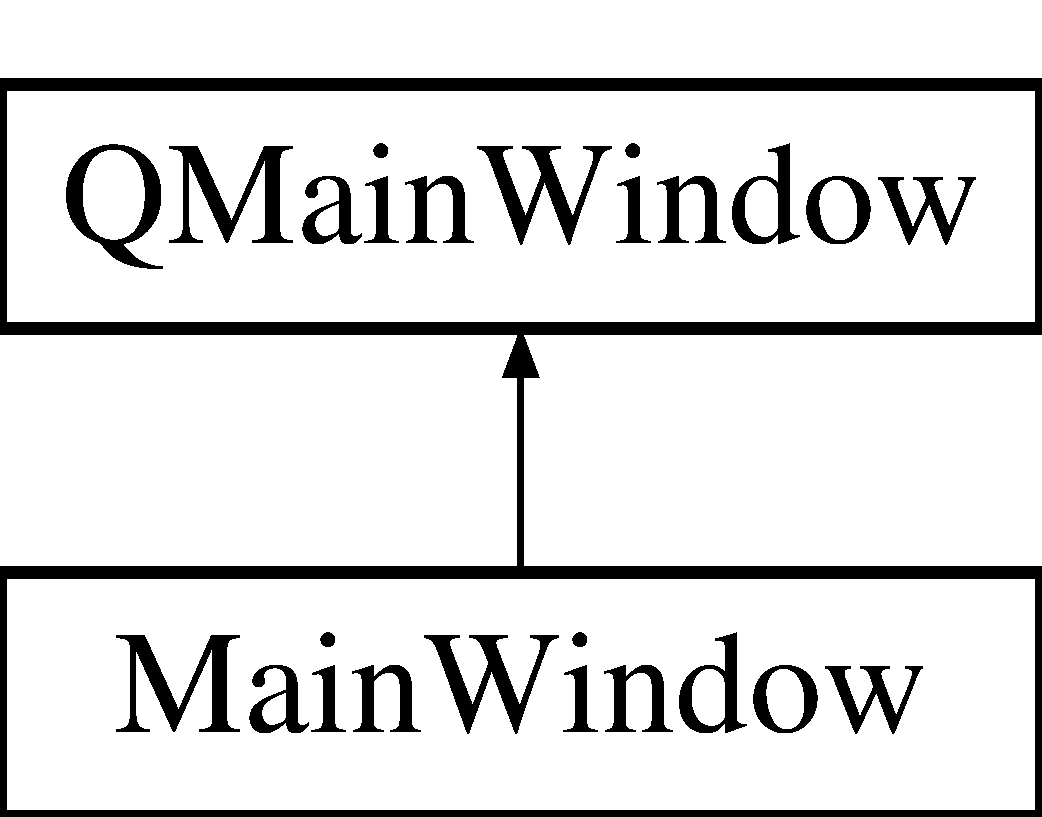
\includegraphics[height=2.000000cm]{class_main_window}
\end{center}
\end{figure}
\subsection*{Public Slots}
\begin{DoxyCompactItemize}
\item 
void \hyperlink{class_main_window_aa0fc566d545a96cb559b8592605b042f}{serial\+Recieved} ()
\begin{DoxyCompactList}\small\item\em fucntion that is executed everytime a serial message is recieved. \end{DoxyCompactList}\item 
void \hyperlink{class_main_window_ae7adeab38af0ac01546badd6baf64270}{send\+Arduino\+Data} (Q\+String)
\begin{DoxyCompactList}\small\item\em send data to arduino via serial bus. \end{DoxyCompactList}\item 
\hypertarget{class_main_window_a4c5237443e9322aa767ef8c307bd2603}{void \hyperlink{class_main_window_a4c5237443e9322aa767ef8c307bd2603}{send\+Arduino\+Data} ()}\label{class_main_window_a4c5237443e9322aa767ef8c307bd2603}

\begin{DoxyCompactList}\small\item\em similar to \hyperlink{class_main_window_ae7adeab38af0ac01546badd6baf64270}{send\+Arduino\+Data(\+Q\+String)}, but sends a null string and act the stream. \end{DoxyCompactList}\end{DoxyCompactItemize}
\subsection*{Signals}
\begin{DoxyCompactItemize}
\item 
void \hyperlink{class_main_window_ab981601bdb64879cd197fb6a6f950e0d}{send\+Arduino} (Q\+String)
\begin{DoxyCompactList}\small\item\em send Arduino string. \end{DoxyCompactList}\item 
void \hyperlink{class_main_window_a5235e26460c2ceee33c224a9d73e6b07}{send\+Arduino} ()
\begin{DoxyCompactList}\small\item\em equivalent to the string counterpart. \end{DoxyCompactList}\item 
\hypertarget{class_main_window_ad00460208b40c79747484b516d1781ce}{void \hyperlink{class_main_window_ad00460208b40c79747484b516d1781ce}{serial\+Recieved\+Processed} ()}\label{class_main_window_ad00460208b40c79747484b516d1781ce}

\begin{DoxyCompactList}\small\item\em signal that indicates that the incoming serial stream has been processed. \end{DoxyCompactList}\item 
\hypertarget{class_main_window_aa3339440163a91fb4a142c18e3c0bd28}{void \hyperlink{class_main_window_aa3339440163a91fb4a142c18e3c0bd28}{serial\+Sent} ()}\label{class_main_window_aa3339440163a91fb4a142c18e3c0bd28}

\begin{DoxyCompactList}\small\item\em signal that indicates that the outgoung serial stream has been processed. \end{DoxyCompactList}\item 
\hypertarget{class_main_window_aac28c5eee22c78e3d3100aa3a0b3926f}{void \hyperlink{class_main_window_aac28c5eee22c78e3d3100aa3a0b3926f}{arduino\+Connection} (bool)}\label{class_main_window_aac28c5eee22c78e3d3100aa3a0b3926f}

\begin{DoxyCompactList}\small\item\em signals that the arduino is connected or not. mainly for G\+U\+I purposes. \end{DoxyCompactList}\item 
\hypertarget{class_main_window_acfedf6f2c7df900495eac711ec3d1f38}{void \hyperlink{class_main_window_acfedf6f2c7df900495eac711ec3d1f38}{motor\+Enable} (bool)}\label{class_main_window_acfedf6f2c7df900495eac711ec3d1f38}

\begin{DoxyCompactList}\small\item\em signals that motor is enabled or not. \end{DoxyCompactList}\item 
\hypertarget{class_main_window_a4ae4250857ad51ba9ee370c7cb5aba10}{void \hyperlink{class_main_window_a4ae4250857ad51ba9ee370c7cb5aba10}{motor\+Output\+C\+W} (bool)}\label{class_main_window_a4ae4250857ad51ba9ee370c7cb5aba10}

\begin{DoxyCompactList}\small\item\em signals that the motor is turning C\+W or C\+C\+W. mainly for G\+U\+I purposes. \end{DoxyCompactList}\item 
void \hyperlink{class_main_window_aa6ffd0e450f99c7c5a7e6f3c0cbc426d}{motor\+Reference\+C\+W} (bool)
\begin{DoxyCompactList}\small\item\em same idea as motor\+Output\+C\+W. \end{DoxyCompactList}\item 
\hypertarget{class_main_window_a56fcae02f5626144c7fd8c84cebcf616}{void \hyperlink{class_main_window_a56fcae02f5626144c7fd8c84cebcf616}{motor\+Stalling} (bool)}\label{class_main_window_a56fcae02f5626144c7fd8c84cebcf616}

\begin{DoxyCompactList}\small\item\em signals if the motor is in intermittent operation. mainly for G\+U\+I purposes. \end{DoxyCompactList}\item 
\hypertarget{class_main_window_aa452712ecfff8368afbb85d733d0c462}{void \hyperlink{class_main_window_aa452712ecfff8368afbb85d733d0c462}{motor\+Output\+R\+P\+M} (Q\+String)}\label{class_main_window_aa452712ecfff8368afbb85d733d0c462}

\begin{DoxyCompactList}\small\item\em used to show a G\+U\+I representation of the arduino output R\+P\+M. \end{DoxyCompactList}\item 
\hypertarget{class_main_window_a95fb9d48208417324b0e1cb6a1f046c8}{void \hyperlink{class_main_window_a95fb9d48208417324b0e1cb6a1f046c8}{motor\+Reference\+R\+P\+M} (Q\+String)}\label{class_main_window_a95fb9d48208417324b0e1cb6a1f046c8}

\begin{DoxyCompactList}\small\item\em used to show a G\+U\+I representation of the arduino reference R\+P\+M. \end{DoxyCompactList}\item 
void \hyperlink{class_main_window_a6c2597367d4174eb49edf2b8f2ecee54}{motor\+Reference\+Recipro\+Freq} (Q\+String)
\begin{DoxyCompactList}\small\item\em simple conversions to frequency. mainly for G\+U\+I purposes. \end{DoxyCompactList}\item 
void \hyperlink{class_main_window_a58e84e8e07511b10f54d838f9b7738a9}{motor\+Output\+Recipro\+Freq} (Q\+String)
\begin{DoxyCompactList}\small\item\em same idea as \hyperlink{class_main_window_a6c2597367d4174eb49edf2b8f2ecee54}{motor\+Reference\+Recipro\+Freq(\+Q\+String)}. \end{DoxyCompactList}\item 
\hypertarget{class_main_window_ae183b93234b45eec5f45ec2d25aceade}{void \hyperlink{class_main_window_ae183b93234b45eec5f45ec2d25aceade}{system\+Height} (Q\+String)}\label{class_main_window_ae183b93234b45eec5f45ec2d25aceade}

\begin{DoxyCompactList}\small\item\em signals the system height given by the arduino serial stream. \end{DoxyCompactList}\item 
\hypertarget{class_main_window_a9394ce562d6dc149df191ec48d1d7d3c}{void \hyperlink{class_main_window_a9394ce562d6dc149df191ec48d1d7d3c}{status\+Message} (Q\+String, int)}\label{class_main_window_a9394ce562d6dc149df191ec48d1d7d3c}

\begin{DoxyCompactList}\small\item\em signal used to show a message into the main windows status bar, with a timer. \end{DoxyCompactList}\item 
\hypertarget{class_main_window_a3ab48045303237d00e9767873f811134}{void \hyperlink{class_main_window_a3ab48045303237d00e9767873f811134}{status\+Message} (Q\+String)}\label{class_main_window_a3ab48045303237d00e9767873f811134}

\begin{DoxyCompactList}\small\item\em same as \hyperlink{class_main_window_a9394ce562d6dc149df191ec48d1d7d3c}{status\+Message(\+Q\+String,int)}, without timer. \end{DoxyCompactList}\end{DoxyCompactItemize}
\subsection*{Public Member Functions}
\begin{DoxyCompactItemize}
\item 
\hypertarget{class_main_window_a8b244be8b7b7db1b08de2a2acb9409db}{\hyperlink{class_main_window_a8b244be8b7b7db1b08de2a2acb9409db}{Main\+Window} (Q\+Widget $\ast$parent=0)}\label{class_main_window_a8b244be8b7b7db1b08de2a2acb9409db}

\begin{DoxyCompactList}\small\item\em default cosntructor \end{DoxyCompactList}\item 
void \hyperlink{class_main_window_a58ed5f08ac0868e866564505ca86ff24}{connect\+Arduino} ()
\begin{DoxyCompactList}\small\item\em the funtion wich tries to connect to and arduino. \end{DoxyCompactList}\end{DoxyCompactItemize}


\subsection{Detailed Description}
The \hyperlink{class_main_window}{Main\+Window} class. Actually is the heart of the interface. All the methods which deal with the arduino itself are coded in the source code of this class. 

\subsection{Member Function Documentation}
\hypertarget{class_main_window_a58ed5f08ac0868e866564505ca86ff24}{\index{Main\+Window@{Main\+Window}!connect\+Arduino@{connect\+Arduino}}
\index{connect\+Arduino@{connect\+Arduino}!Main\+Window@{Main\+Window}}
\subsubsection[{connect\+Arduino}]{\setlength{\rightskip}{0pt plus 5cm}void Main\+Window\+::connect\+Arduino (
\begin{DoxyParamCaption}
{}
\end{DoxyParamCaption}
)}}\label{class_main_window_a58ed5f08ac0868e866564505ca86ff24}


the funtion wich tries to connect to and arduino. 

This function tries to be as cross-\/platform possible, by iterating in the lsit given by the Qt\+Serial library and attempting connection with the first possibility it finds. There is a draw back to this approach\+: The assumption that only on arduino is connected to the machine.

By calling the function the internal variable serial is manipulated in this respect. \hypertarget{class_main_window_a58e84e8e07511b10f54d838f9b7738a9}{\index{Main\+Window@{Main\+Window}!motor\+Output\+Recipro\+Freq@{motor\+Output\+Recipro\+Freq}}
\index{motor\+Output\+Recipro\+Freq@{motor\+Output\+Recipro\+Freq}!Main\+Window@{Main\+Window}}
\subsubsection[{motor\+Output\+Recipro\+Freq}]{\setlength{\rightskip}{0pt plus 5cm}void Main\+Window\+::motor\+Output\+Recipro\+Freq (
\begin{DoxyParamCaption}
\item[{Q\+String}]{}
\end{DoxyParamCaption}
)\hspace{0.3cm}{\ttfamily [signal]}}}\label{class_main_window_a58e84e8e07511b10f54d838f9b7738a9}


same idea as \hyperlink{class_main_window_a6c2597367d4174eb49edf2b8f2ecee54}{motor\+Reference\+Recipro\+Freq(\+Q\+String)}. 

\begin{DoxySeeAlso}{See also}
\hyperlink{class_main_window_aa452712ecfff8368afbb85d733d0c462}{motor\+Output\+R\+P\+M(\+Q\+String)} 
\end{DoxySeeAlso}
\hypertarget{class_main_window_aa6ffd0e450f99c7c5a7e6f3c0cbc426d}{\index{Main\+Window@{Main\+Window}!motor\+Reference\+C\+W@{motor\+Reference\+C\+W}}
\index{motor\+Reference\+C\+W@{motor\+Reference\+C\+W}!Main\+Window@{Main\+Window}}
\subsubsection[{motor\+Reference\+C\+W}]{\setlength{\rightskip}{0pt plus 5cm}void Main\+Window\+::motor\+Reference\+C\+W (
\begin{DoxyParamCaption}
\item[{bool}]{}
\end{DoxyParamCaption}
)\hspace{0.3cm}{\ttfamily [signal]}}}\label{class_main_window_aa6ffd0e450f99c7c5a7e6f3c0cbc426d}


same idea as motor\+Output\+C\+W. 

\begin{DoxySeeAlso}{See also}
\hyperlink{class_main_window_a4ae4250857ad51ba9ee370c7cb5aba10}{motor\+Output\+C\+W(bool)} 
\end{DoxySeeAlso}
\hypertarget{class_main_window_a6c2597367d4174eb49edf2b8f2ecee54}{\index{Main\+Window@{Main\+Window}!motor\+Reference\+Recipro\+Freq@{motor\+Reference\+Recipro\+Freq}}
\index{motor\+Reference\+Recipro\+Freq@{motor\+Reference\+Recipro\+Freq}!Main\+Window@{Main\+Window}}
\subsubsection[{motor\+Reference\+Recipro\+Freq}]{\setlength{\rightskip}{0pt plus 5cm}void Main\+Window\+::motor\+Reference\+Recipro\+Freq (
\begin{DoxyParamCaption}
\item[{Q\+String}]{}
\end{DoxyParamCaption}
)\hspace{0.3cm}{\ttfamily [signal]}}}\label{class_main_window_a6c2597367d4174eb49edf2b8f2ecee54}


simple conversions to frequency. mainly for G\+U\+I purposes. 

\begin{DoxySeeAlso}{See also}
motor\+Reference\+R\+P\+M(\+Qstring) 
\end{DoxySeeAlso}
\hypertarget{class_main_window_ab981601bdb64879cd197fb6a6f950e0d}{\index{Main\+Window@{Main\+Window}!send\+Arduino@{send\+Arduino}}
\index{send\+Arduino@{send\+Arduino}!Main\+Window@{Main\+Window}}
\subsubsection[{send\+Arduino}]{\setlength{\rightskip}{0pt plus 5cm}void Main\+Window\+::send\+Arduino (
\begin{DoxyParamCaption}
\item[{Q\+String}]{}
\end{DoxyParamCaption}
)\hspace{0.3cm}{\ttfamily [signal]}}}\label{class_main_window_ab981601bdb64879cd197fb6a6f950e0d}


send Arduino string. 

The signal to send Arduino any commands and numbers within the string. If the arduino is not connect, however, a message is printed into the status bar telling that the arduino is not connected and no action takes place. \hypertarget{class_main_window_a5235e26460c2ceee33c224a9d73e6b07}{\index{Main\+Window@{Main\+Window}!send\+Arduino@{send\+Arduino}}
\index{send\+Arduino@{send\+Arduino}!Main\+Window@{Main\+Window}}
\subsubsection[{send\+Arduino}]{\setlength{\rightskip}{0pt plus 5cm}void Main\+Window\+::send\+Arduino (
\begin{DoxyParamCaption}
{}
\end{DoxyParamCaption}
)\hspace{0.3cm}{\ttfamily [signal]}}}\label{class_main_window_a5235e26460c2ceee33c224a9d73e6b07}


equivalent to the string counterpart. 

\begin{DoxySeeAlso}{See also}
\hyperlink{class_main_window_ab981601bdb64879cd197fb6a6f950e0d}{send\+Arduino(\+Q\+String)}; 
\end{DoxySeeAlso}
\hypertarget{class_main_window_ae7adeab38af0ac01546badd6baf64270}{\index{Main\+Window@{Main\+Window}!send\+Arduino\+Data@{send\+Arduino\+Data}}
\index{send\+Arduino\+Data@{send\+Arduino\+Data}!Main\+Window@{Main\+Window}}
\subsubsection[{send\+Arduino\+Data}]{\setlength{\rightskip}{0pt plus 5cm}void Main\+Window\+::send\+Arduino\+Data (
\begin{DoxyParamCaption}
\item[{Q\+String}]{data}
\end{DoxyParamCaption}
)\hspace{0.3cm}{\ttfamily [slot]}}}\label{class_main_window_ae7adeab38af0ac01546badd6baf64270}


send data to arduino via serial bus. 

Takes the string given in the slot and sends it in the correct form to the arduino via serial bus. The string can be any command that the arduino recognizes (invalid commands and chars are ignored by the arduino internal parser).

If the serial is still being processes; the string is appended to the end of the outgoing stream. \hypertarget{class_main_window_aa0fc566d545a96cb559b8592605b042f}{\index{Main\+Window@{Main\+Window}!serial\+Recieved@{serial\+Recieved}}
\index{serial\+Recieved@{serial\+Recieved}!Main\+Window@{Main\+Window}}
\subsubsection[{serial\+Recieved}]{\setlength{\rightskip}{0pt plus 5cm}void Main\+Window\+::serial\+Recieved (
\begin{DoxyParamCaption}
{}
\end{DoxyParamCaption}
)\hspace{0.3cm}{\ttfamily [slot]}}}\label{class_main_window_aa0fc566d545a96cb559b8592605b042f}


fucntion that is executed everytime a serial message is recieved. 

This function processes all the serial data recieved by the Arduino. Since it does not behave like the arduino processing does, being faster in this respect; a internal buffer is necessary to gather all the data until a linefeed is issued. If this happens, the buffer is taken and processed according to the minimal standard adopted in the arduino\+:

Enabled; Stalling; reference R\+P\+M; output R\+P\+M; output Height; 

The documentation for this class was generated from the following files\+:\begin{DoxyCompactItemize}
\item 
mainwindow.\+h\item 
mainwindow.\+cpp\end{DoxyCompactItemize}

\hypertarget{classprogress_dialog}{\section{progress\+Dialog Class Reference}
\label{classprogress_dialog}\index{progress\+Dialog@{progress\+Dialog}}
}


The \hyperlink{classprogress_dialog}{progress\+Dialog} class is a simple progress bar for value recording.  




{\ttfamily \#include $<$progressdialog.\+h$>$}

Inheritance diagram for progress\+Dialog\+:\begin{figure}[H]
\begin{center}
\leavevmode
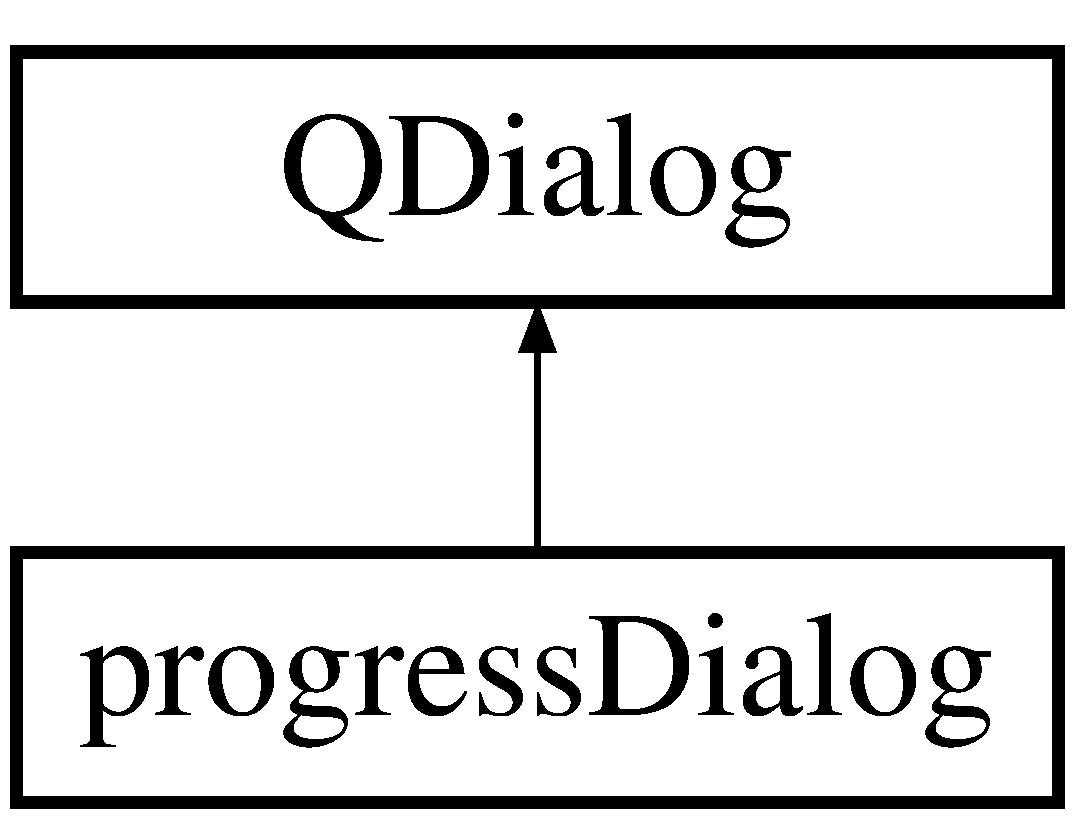
\includegraphics[height=2.000000cm]{classprogress_dialog}
\end{center}
\end{figure}
\subsection*{Public Slots}
\begin{DoxyCompactItemize}
\item 
void \hyperlink{classprogress_dialog_ac6b3d582453f56d5f86758bbef380e52}{record\+Value} (double)
\begin{DoxyCompactList}\small\item\em tkae a double value and add it to the stack. \end{DoxyCompactList}\item 
void \hyperlink{classprogress_dialog_acf8d15fdaea84dd2cfb07305aa973776}{record\+Value} (Q\+String)
\begin{DoxyCompactList}\small\item\em record\+Value placeholder. \end{DoxyCompactList}\end{DoxyCompactItemize}
\subsection*{Signals}
\begin{DoxyCompactItemize}
\item 
void \hyperlink{classprogress_dialog_ab5054e13998ff01af0fa74c5703365d0}{set\+Progress} (int)
\begin{DoxyCompactList}\small\item\em simple G\+U\+I fucntion. \end{DoxyCompactList}\end{DoxyCompactItemize}
\subsection*{Public Member Functions}
\begin{DoxyCompactItemize}
\item 
\hyperlink{classprogress_dialog_a95133b1accf321c0a30a9cd27605c907}{progress\+Dialog} (Q\+Widget $\ast$parent=0, int dim\+\_\+=50, Q\+String tracked=\char`\"{}\char`\"{})
\begin{DoxyCompactList}\small\item\em \hyperlink{classprogress_dialog}{progress\+Dialog} constructor. \end{DoxyCompactList}\end{DoxyCompactItemize}


\subsection{Detailed Description}
The \hyperlink{classprogress_dialog}{progress\+Dialog} class is a simple progress bar for value recording. 

This class manages both the gui representing the value recording and the recording itself, by storing the samples internally. The sample size is given in the class construction.

The recording itself happens via slots from the mainwindow to one instance of this class. 

\subsection{Constructor \& Destructor Documentation}
\hypertarget{classprogress_dialog_a95133b1accf321c0a30a9cd27605c907}{\index{progress\+Dialog@{progress\+Dialog}!progress\+Dialog@{progress\+Dialog}}
\index{progress\+Dialog@{progress\+Dialog}!progress\+Dialog@{progress\+Dialog}}
\subsubsection[{progress\+Dialog}]{\setlength{\rightskip}{0pt plus 5cm}progress\+Dialog\+::progress\+Dialog (
\begin{DoxyParamCaption}
\item[{Q\+Widget $\ast$}]{parent = {\ttfamily 0}, }
\item[{int}]{dim\+\_\+ = {\ttfamily 50}, }
\item[{Q\+String}]{tracked = {\ttfamily \char`\"{}\char`\"{}}}
\end{DoxyParamCaption}
)\hspace{0.3cm}{\ttfamily [explicit]}}}\label{classprogress_dialog_a95133b1accf321c0a30a9cd27605c907}


\hyperlink{classprogress_dialog}{progress\+Dialog} constructor. 

The constructor must recieve the sample size which it will record so that the sample size can be tracked and managed internally. The name of the title should also be given for aesthetics.


\begin{DoxyParams}{Parameters}
{\em parent} & generally the main window. \\
\hline
{\em dim\+\_\+} & the samplign size that the object will manage. \\
\hline
{\em tracked} & the actual title of the G\+U\+I. \\
\hline
\end{DoxyParams}


\subsection{Member Function Documentation}
\hypertarget{classprogress_dialog_ac6b3d582453f56d5f86758bbef380e52}{\index{progress\+Dialog@{progress\+Dialog}!record\+Value@{record\+Value}}
\index{record\+Value@{record\+Value}!progress\+Dialog@{progress\+Dialog}}
\subsubsection[{record\+Value}]{\setlength{\rightskip}{0pt plus 5cm}void progress\+Dialog\+::record\+Value (
\begin{DoxyParamCaption}
\item[{double}]{value}
\end{DoxyParamCaption}
)\hspace{0.3cm}{\ttfamily [slot]}}}\label{classprogress_dialog_ac6b3d582453f56d5f86758bbef380e52}


tkae a double value and add it to the stack. 

take the double given in the signal and add it to the internal sampel stack, managing the G\+U\+I and internal variables automatically. When the stack reaches the desired sample size, a finished signal is emited and a prompt for save is given. \hypertarget{classprogress_dialog_acf8d15fdaea84dd2cfb07305aa973776}{\index{progress\+Dialog@{progress\+Dialog}!record\+Value@{record\+Value}}
\index{record\+Value@{record\+Value}!progress\+Dialog@{progress\+Dialog}}
\subsubsection[{record\+Value}]{\setlength{\rightskip}{0pt plus 5cm}void progress\+Dialog\+::record\+Value (
\begin{DoxyParamCaption}
\item[{Q\+String}]{value}
\end{DoxyParamCaption}
)\hspace{0.3cm}{\ttfamily [slot]}}}\label{classprogress_dialog_acf8d15fdaea84dd2cfb07305aa973776}


record\+Value placeholder. 

This signal is a placeholder for the record\+Value signal, which tries to convert the string to double format and the calls the correct \hyperlink{classprogress_dialog_ac6b3d582453f56d5f86758bbef380e52}{record\+Value(double)}. \hypertarget{classprogress_dialog_ab5054e13998ff01af0fa74c5703365d0}{\index{progress\+Dialog@{progress\+Dialog}!set\+Progress@{set\+Progress}}
\index{set\+Progress@{set\+Progress}!progress\+Dialog@{progress\+Dialog}}
\subsubsection[{set\+Progress}]{\setlength{\rightskip}{0pt plus 5cm}void progress\+Dialog\+::set\+Progress (
\begin{DoxyParamCaption}
\item[{int}]{}
\end{DoxyParamCaption}
)\hspace{0.3cm}{\ttfamily [signal]}}}\label{classprogress_dialog_ab5054e13998ff01af0fa74c5703365d0}


simple G\+U\+I fucntion. 

This takes an int and represent it accordingly into the progress bar, making it show another percentage. 

The documentation for this class was generated from the following files\+:\begin{DoxyCompactItemize}
\item 
progressdialog.\+h\item 
progressdialog.\+cpp\end{DoxyCompactItemize}

\hypertarget{class_variable_editor}{\section{Variable\+Editor Class Reference}
\label{class_variable_editor}\index{Variable\+Editor@{Variable\+Editor}}
}


The \hyperlink{class_variable_editor}{Variable\+Editor} class is a simple global internal variable editor.  




{\ttfamily \#include $<$variableeditor.\+h$>$}

Inheritance diagram for Variable\+Editor\+:\begin{figure}[H]
\begin{center}
\leavevmode
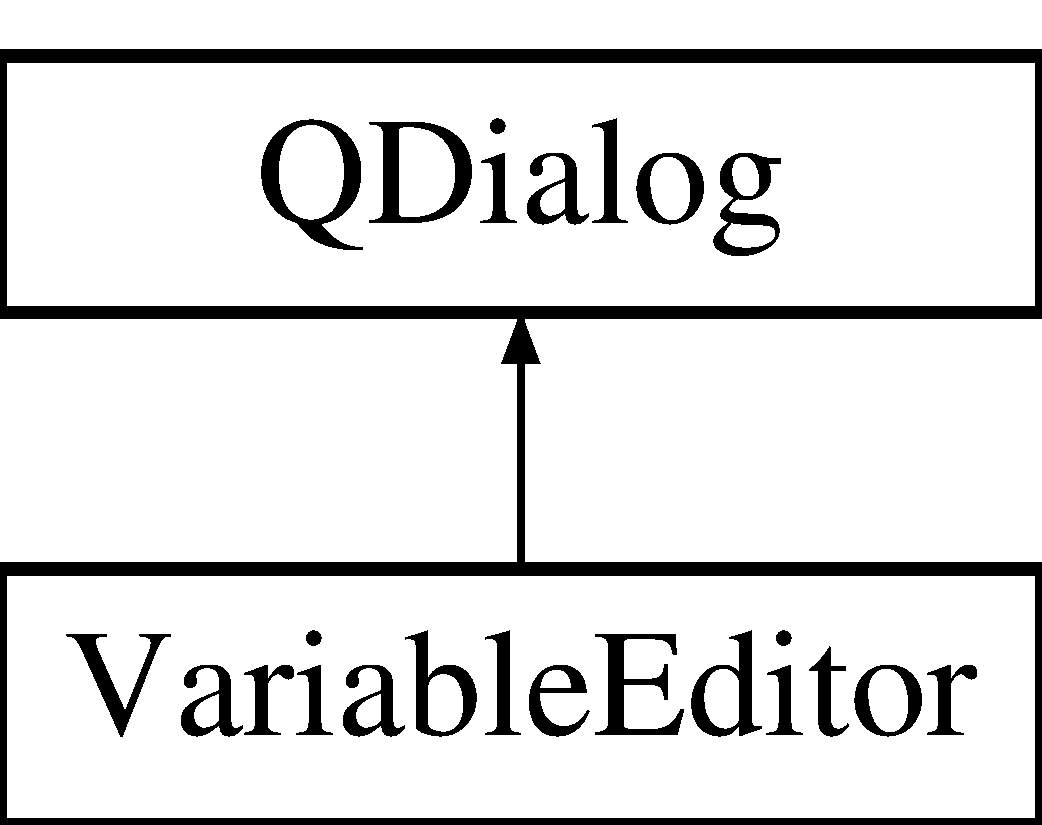
\includegraphics[height=2.000000cm]{class_variable_editor}
\end{center}
\end{figure}
\subsection*{Signals}
\begin{DoxyCompactItemize}
\item 
void \hyperlink{class_variable_editor_ad63cad542a41c66adf493666a531f1e3}{s\+\_\+set\+Vars} (Q\+List$<$ int $>$, Q\+List$<$ double $>$)
\begin{DoxyCompactList}\small\item\em s\+\_\+set\+Vars signals the new variables to be set in the main window. \end{DoxyCompactList}\end{DoxyCompactItemize}
\subsection*{Public Member Functions}
\begin{DoxyCompactItemize}
\item 
\hyperlink{class_variable_editor_a06fa8d1cdccf80a0a9fc9a706380f5ef}{Variable\+Editor} (Q\+Widget $\ast$parent=0, Q\+List$<$ int $>$ int\+\_\+vars\+\_\+=Q\+List$<$ int $>$(), Q\+List$<$ double $>$ double\+\_\+vars\+\_\+=Q\+List$<$ double $>$())
\begin{DoxyCompactList}\small\item\em \hyperlink{class_variable_editor}{Variable\+Editor} contructor, needs a couple of parameters. \end{DoxyCompactList}\end{DoxyCompactItemize}


\subsection{Detailed Description}
The \hyperlink{class_variable_editor}{Variable\+Editor} class is a simple global internal variable editor. 

The goal is that the object created changes the global variables determined into the mainwindow such as sample size and height extrema. 

\subsection{Constructor \& Destructor Documentation}
\hypertarget{class_variable_editor_a06fa8d1cdccf80a0a9fc9a706380f5ef}{\index{Variable\+Editor@{Variable\+Editor}!Variable\+Editor@{Variable\+Editor}}
\index{Variable\+Editor@{Variable\+Editor}!Variable\+Editor@{Variable\+Editor}}
\subsubsection[{Variable\+Editor}]{\setlength{\rightskip}{0pt plus 5cm}Variable\+Editor\+::\+Variable\+Editor (
\begin{DoxyParamCaption}
\item[{Q\+Widget $\ast$}]{parent = {\ttfamily 0}, }
\item[{Q\+List$<$ int $>$}]{int\+\_\+vars\+\_\+ = {\ttfamily QList$<$int$>$()}, }
\item[{Q\+List$<$ double $>$}]{double\+\_\+vars\+\_\+ = {\ttfamily QList$<$double$>$()}}
\end{DoxyParamCaption}
)\hspace{0.3cm}{\ttfamily [explicit]}}}\label{class_variable_editor_a06fa8d1cdccf80a0a9fc9a706380f5ef}


\hyperlink{class_variable_editor}{Variable\+Editor} contructor, needs a couple of parameters. 

To make the variables appear in the correct way, they are passed as lists by the mainwindow object and then processed internally by this class.

Although the numbering and rows managning is automatic, the row labels are not. If more global variables are defined and need to be managed, the source code must be modified accordingly, in this class and in the \hyperlink{class_main_window}{Main\+Window} class.


\begin{DoxyParams}{Parameters}
{\em parent} & The usual G\+U\+I parent. Genrally the mainwindow. \\
\hline
{\em int\+\_\+vars\+\_\+} & the input list of integer variables. \\
\hline
{\em double\+\_\+vars\+\_\+} & the input list of double/float variables. \\
\hline
\end{DoxyParams}


\subsection{Member Function Documentation}
\hypertarget{class_variable_editor_ad63cad542a41c66adf493666a531f1e3}{\index{Variable\+Editor@{Variable\+Editor}!s\+\_\+set\+Vars@{s\+\_\+set\+Vars}}
\index{s\+\_\+set\+Vars@{s\+\_\+set\+Vars}!Variable\+Editor@{Variable\+Editor}}
\subsubsection[{s\+\_\+set\+Vars}]{\setlength{\rightskip}{0pt plus 5cm}void Variable\+Editor\+::s\+\_\+set\+Vars (
\begin{DoxyParamCaption}
\item[{Q\+List$<$ int $>$}]{, }
\item[{Q\+List$<$ double $>$}]{}
\end{DoxyParamCaption}
)\hspace{0.3cm}{\ttfamily [signal]}}}\label{class_variable_editor_ad63cad542a41c66adf493666a531f1e3}


s\+\_\+set\+Vars signals the new variables to be set in the main window. 

The variable chaging is not entirelly general in the mainwindow class and if a new global variable is created and needs to be managed, as stated in \hyperlink{class_variable_editor_a06fa8d1cdccf80a0a9fc9a706380f5ef}{Variable\+Editor()} description;the correspondent source code of the \hyperlink{class_main_window}{Main\+Window} class also needs to be changed. Although it is a straighforward change. 

The documentation for this class was generated from the following files\+:\begin{DoxyCompactItemize}
\item 
variableeditor.\+h\item 
variableeditor.\+cpp\end{DoxyCompactItemize}

%--- End generated contents ---

% Index
\newpage
\phantomsection
\addcontentsline{toc}{chapter}{Index}
\printindex

\end{document}
